\chapter{Apéndice}
\section{bot.php}
Código que hace la inserción a CRM
\begin{minted}{php}
<?php
if(isset($_POST['chatfuel'])){
  if($_POST['chatfuel'] == "8cuNbZVtDgYJvkdzYbohnPiY"){
    $_POST['system_id'] = (int)$_POST['system_id'];
    /Translate/
    $_POST['first_name'] = $_POST['fb_first_name']." ".$_POST['fb_last_name'];
    $_POST['phone']     = str_replace(" ","",$_POST['phone']);
    $_POST['phone']     = substr($_POST['phone'],0,10);
    $_POST['landing'] = $_POST['ad_content'];
    $_POST['months_behind'] = str_replace(" meses","",$_POST['meses']);
    $_POST['borrower_insitute'] = $_POST['acredores'];
    $_POST['borrower_insitute'] = $_POST['acredores'];

    /Validation and fix/
    if(!preg_match('/./',$_POST['email'])){
        $_POST['email'] = $_POST['email'].'.com';
    }

    if(filter_var($_POST['email'], FILTER_VALIDATE_EMAIL)) {
    }else{
      $datetime = date("Y_m_d_H_i_s");
      $_POST['email'] = $datetime."@unknown-mail.com";
    }

    function toASCII( $str ){
        return strtr(utf8_decode($str), 
            utf8_decode(
            'ŠŒŽšœžŸ¥µÀÁ ÃÄÅÆÇÈÉÊËÌÍÎÏÐÑÒÓÔÕÖØÙÚÛÜÝßàáâãäåæçèéêëìíîïðñòóôõöøùúûüýÿ'),
            'SOZsozYYuAAAAAAACEEEEIIIIDNOOOOOOUUUUYsaaaaaaaceeeeiiiionoooooouuuuyy');
    }

    $_POST['email']       = toASCII($_POST['email']);
    $_POST['debt_amount'] = str_replace(",","",$_POST['debt_amount']);

    /Unset old values/
    unset($_POST['fb_first_name']);
    unset($_POST['fb_last_name']);
    unset($_POST['ad_content']);
    unset($_POST['meses']);
    unset($_POST['acredores']);
    unset($_POST['chatfuel']);

    /Transform to json/
    $data=json_encode($_POST);
    
    /Test or production/
    $url = 'https://urmdamghr3.execute-api.us-east-1.amazonaws.com/prod/Leads/registerLead';

    $ch = curl_init( $url );
    curl_setopt( $ch, CURLOPT_POST, 1);
    curl_setopt( $ch, CURLOPT_POSTFIELDS, $data);
    curl_setopt( $ch, CURLOPT_FOLLOWLOCATION, 1);
    curl_setopt( $ch, CURLOPT_HEADER, 0);
    curl_setopt( $ch, CURLOPT_RETURNTRANSFER, 1);

    $response = curl_exec( $ch );
  }
}
print_r("v0.3");
exit("");\end{minted}

\section{calculaDescuento.py}
Código que calcula el descuento de los clientes
\begin{minted}[mathescape,gobble=2]{python}
  # coding: utf-8
from __future__ import print_function
import json
import sys
import boto3


print('Loading function')

#event={"institucion": sys.argv[1],"deuda":sys.argv[2],"atraso":sys.argv[3]}
ins=event['institucion']
deuda=round(float((event['deuda'])))
atraso=int(event['atraso'])
descuento=0



def lambda_handler(event, context):    
    """Ejecuta el cálculo del descuento
    Argumentos:
    event -- datos del usuario para cálculo del descuento(dict)
    context --  variables de entorno(str)"""
    print("Parametros recibidos: ")
    print("Institucion= "+ins)
    print("Deuda= " + str(deuda))
    print("Atraso= "+str(atraso))
    
    nuevodescuento=calculaDescuento(ins,atraso)
    print ("Nuevo Descuento="+ str(nuevodescuento))

    nuevadeuda = round(deuda*.01*nuevodescuento)
    print("Nueva deuda="+str(nuevadeuda))
    #nuevadeuda=calculaDescuento(ins,deuda,atraso)
    mensaje1='Tu deuda de $'+ str(deuda)+' con ' +ins+" con atraso de "+ str(atraso)+" meses"
    mensaje2='Quedaria en $'+ str(nuevadeuda)
    print(mensaje1)
    print(mensaje2)

    not_encoded=[{"text": mensaje1},{"text": mensaje2}]
    res=json.dumps(not_encoded)
    
    return(not_encoded)







"""Métodos para calcular descuento
Argumentos:
atraso: meses de atraso(int)"""
descuento=0
def descuentoBancomer(atraso):
    if atraso==1:
            descuento=15
    elif atraso==2:
            descuento=32
    elif atraso==3:
            descuento=48
    elif atraso==4:
            descuento=60
    elif atraso==5:
            descuento=67
    elif atraso>=6:
            descuento=85
    return descuento

def descuentoBanamex(atraso):
    if atraso>=0 and atraso<=4:
        descuento=0
    elif atraso==5:
        descuento=57
    elif atraso==6:
        descuento=62
    elif atraso==7:
        descuento=66
    elif atraso==8 or atraso==9:
        descuento=70
    elif atraso>=6:
        print (str(atraso) +" es mayor a 6")
        descuento=74
        print("entonces descuento="+str(descuento))
    return descuento

def descuentoAmex(atraso):
    if atraso>=0 and atraso<=2:
        descuento=0
    elif atraso==3:
        descuento=5
    elif atraso>=4:
        descuento=25
    return descuento

def descuentoBanorte(atraso):            
    if atraso>=0 and atraso<=4:
        descuento=5
    elif atraso>=5 and atraso<=8:
        descuento=40
    elif atraso>=9:
        descuento=55
    return descuento

def descuentoHSBC(atraso):
    if atraso>=0 and atraso<=2:
        descuento=0,
    elif atraso>=3 and atraso<=4:
        descuento=40,
    elif atraso>=5 and atraso<=6:
        descuento=50,
    elif atraso>6:
        descuento=60
    return descuento

def descuentoScotiabank(atraso):
    if atraso>=0 and atraso<=4:
        descuento=0,
    elif atraso>4:
        descuento=45
    return descuento
def descuentoGlobal(atraso):
    if atraso>=0 and atraso<=4:
        descuento=0
    elif atraso>4:
        descuento=45
    return descuento

def descuentoInbursa(atraso):
    if atraso>=0 and atraso<=4:
        descuento=45
    elif atraso>4:
        descuento=50
    return descuento 



def descuentoCA(atraso):
    if atraso>=1 and  atraso<=4:
        descuento=0
    elif atraso>4:
        descuento=10
    return descuento

def descuentoIxe(atraso):
    if atraso<5:
        descuento=0
    elif atraso>=5:
        descuento=30
    return descuento

def descuentoInvex(atraso):
    if atraso>=0 and atraso<=2:
        descuento=0
    elif atraso==3:
        descuento=35
    elif atraso>=4:
        descuento=45
    return descuento

def descuentoCredFamiliar(atraso):
    if atraso >=1 and atraso<=4: 
        descuento=0
    elif atraso>=5:
        descuento=35
    return descuento

def descuentoSantander(atraso):
    if atraso==1:
         descuento=10
    elif atraso==2:
        descuento=20
    elif atraso==3:
        descuento=30
    elif atraso==4:
        desceunto=50
    elif atraso>=5:
        descuento=55
    return descuento

def descuentoSantander(atraso):
    if atraso==1:
        descuento=10
    elif atraso==2:
        descuento=20
    elif atraso==3:
        descuento=30
    elif atraso==4:
        desceunto=50
    elif atraso>=5:
        descuento=55
    return descuento

def descuentoPH(atraso):
    if atraso>4:
        descuento=15
    return descuento

def descuentoSears(atraso):
    if atraso>4:
        descuento=15
    return descuento

def descuentoCredomatic(atraso):
    if atraso >=1 and atraso<=4:
        descuento=0
    elif atraso>=5 and atraso<=6:
        descuento=10
    elif atraso>6:
        descuento=20
    return descuento

def descuentoWalmart(atraso):
    if atraso>=1 and atraso<=4:
        descuento=0
    elif atraso>=5 and atraso<=6:
        descuento=10
    elif atraso>6:
        descuento=20
    return descuento
def descuentoLiverpool(atraso):
    if atraso>=1 and atraso<=4:
        descuento=0
    elif atraso>=5 and atraso<=6:
        descuento=10
    elif atraso>6:
        descuento=20
    return descuento

def calculaDescuento(ins, atraso):
    """calcula el total a pagar con el descuento
    Argumentos:
    ins -- institucion a la que se le debe(str)
    atraso -- meses pago atrasado(int)"""
    switcher = {
            "Bancomer": descuentoBancomer(atraso),
            "Banamex": descuentoBanamex(atraso),
            "AMEX": descuentoAmex(atraso),
            "Banorte":descuentoBanorte(atraso),
            "HSBC":descuentoHSBC(atraso),
            "Scotiabank":descuentoScotiabank(atraso),
            "Global":descuentoGlobal(atraso),
            "Inbursa":descuentoInbursa(atraso),
            "Liverpool":descuentoLiverpool(atraso),
            "C&A":descuentoCA(atraso),
            "IXE":descuentoIxe(atraso),
            "Invex":descuentoInvex(atraso),
            "Credito Familiar":descuentoCredFamiliar(atraso),
            "Santander":descuentoSantander(atraso),
            "Palacio de Hierro":descuentoPH(atraso),
            "Sears":descuentoSears(atraso),
            "Credomatic":descuentoCredomatic(atraso),
            "Walmart":descuentoWalmart(atraso),
             2: lambda: "two",
    
        }
    func = switcher.get(ins, lambda: "nothing")
    
    # Execute the function
    return func



lambda_handler(event,1)

\end{minted}
\chapter{Imagenes} 
Time Lag - días desde que se produce la primera interacción hasta que se produce la conversión
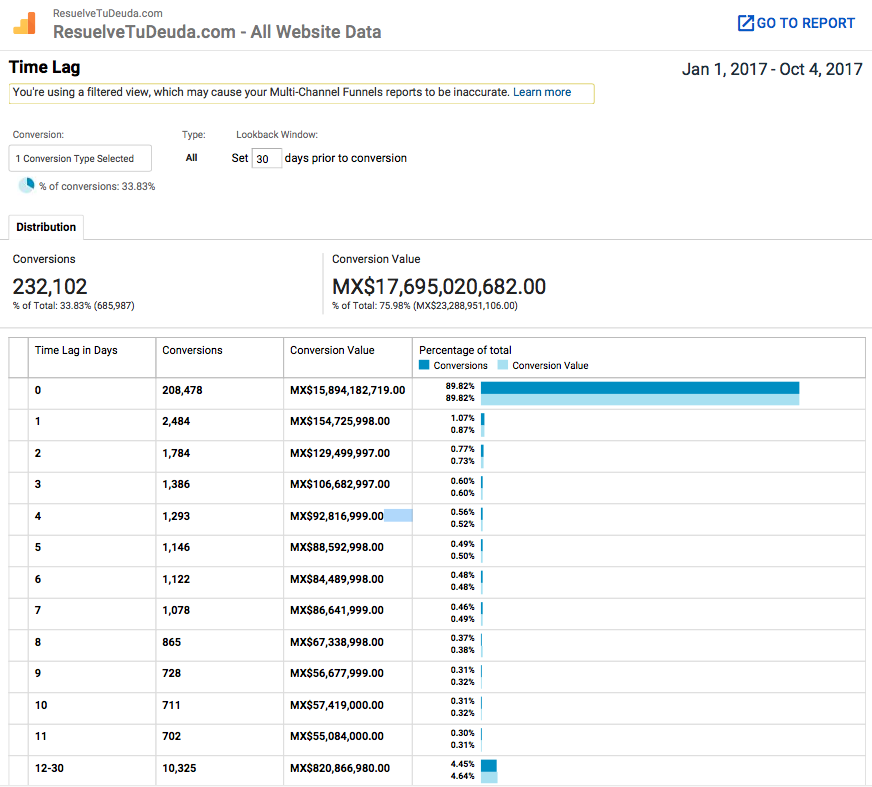
\includegraphics[width=\textwidth]{TimeLag.jpg}
